\documentclass[compress]{beamer}
\usepackage{ifthen,verbatim}

\newcommand{\isnote}{}
\xdefinecolor{lightyellow}{rgb}{1.,1.,0.25}
\xdefinecolor{darkblue}{rgb}{0.1,0.1,0.7}

%% Uncomment this to get annotations
%% \def\notes{\addtocounter{page}{-1}
%%            \renewcommand{\isnote}{*}
%% 	   \beamertemplateshadingbackground{lightyellow}{white}
%%            \begin{frame}
%%            \frametitle{Notes for the previous page (page \insertpagenumber)}
%%            \itemize}
%% \def\endnotes{\enditemize
%% 	      \end{frame}
%%               \beamertemplateshadingbackground{white}{white}
%%               \renewcommand{\isnote}{}}

%% Uncomment this to not get annotations
\def\notes{\comment}
\def\endnotes{\endcomment}

\setbeamertemplate{navigation symbols}{}
\setbeamertemplate{headline}{\mbox{ } \hfill
\begin{minipage}{5.5 cm}
\vspace{-0.75 cm} \small
\end{minipage} \hfill
\begin{minipage}{4.5 cm}
\vspace{-0.75 cm} \small
\begin{flushright}
\ifthenelse{\equal{\insertpagenumber}{1}}{}{Jim Pivarski \hspace{0.2 cm} \insertpagenumber\isnote/\pageref{numpages}}
\end{flushright}
\end{minipage}\mbox{\hspace{0.2 cm}}\includegraphics[height=1 cm]{../cmslogo} \hspace{0.1 cm} \includegraphics[height=1 cm]{../tamulogo} \hspace{0.01 cm} \vspace{-1.05 cm}}

\begin{document}
\begin{frame}
\vfill
\begin{center}
\textcolor{darkblue}{\Large Follow-up Studies in Track-Based Muon Alignment}

\vfill
\begin{columns}
\column{0.3\linewidth}
\begin{center}
\large
\textcolor{darkblue}{Jim Pivarski}

\vspace{0.2 cm}
Alexei Safonov
\end{center}
\end{columns}

\begin{columns}
\column{0.3\linewidth}
\begin{center}
\scriptsize
{\it Texas A\&M University}
\end{center}
\end{columns}

\vfill
25 November, 2008

\end{center}
\end{frame}

%% \begin{notes}
%% \item This is the annotated version of my talk.
%% \item If you want the version that I am presenting, download the one
%% labeled ``slides'' on Indico (or just ignore these yellow pages).
%% \item The annotated version is provided for extra detail and a written
%% record of comments that I intend to make orally.
%% \item Yellow notes refer to the content on the {\it previous} page.
%% \item All other slides are identical for the two versions.
%% \end{notes}

\small

\begin{frame}
\frametitle{Background and motivation}
\begin{itemize}\setlength{\itemsep}{0.1 cm}
\item First attempt at track-based muon alignments were presented by both
  algorithms (HIP and MillePede), showing rough agreement with each
  other, but not with expectations
\item Questions raised:
\begin{itemize}
\item are there really 2--3~mrad rotations in the minus muon endcap?
\item why is the $z$ compression so much larger in track-based alignment than expected?
\item are there biases coming from the tracker's weak modes
  ($\chi^2$-invariant global distortions)?
\end{itemize}

\item Track-based muon alignment not used for first \mbox{CRAFT re-processing\hspace{-1 cm}}

\item The dataset is huge; we should be able to answer some of these
  questions by slicing it up appropriately

\item These slides partially answer the above questions
\begin{itemize}
\item by studying the tracks in more detail
\item by applying trial distortions to the tracker, to quantify
  sensitivity of muon alignment to these weak modes
\end{itemize}
\end{itemize}
%% \hspace{-0.83 cm} \textcolor{darkblue}{\Large Outline2}
\end{frame}

\begin{frame}
\frametitle{Slicing up the dataset}
\begin{itemize}\setlength{\itemsep}{0.1 cm}
\item Track-based procedure treats each wheel/disk as one bin \mbox{for averages\hspace{-1 cm}}
\item With $10^{4\mbox{-}5}$ globalMuons in the barrel, we can afford smaller bins
\item Plot the same muon residuals as a function of (1) muon hit position
  and (2) Point of Closest Approach (PCA) to beamline, \mbox{in the tracker\hspace{-1 cm}}
\begin{itemize}
\item muon misalignments will show up as steps in $Z_{\mbox{\scriptsize muon}}$;
  tracker misalignments will make strong trends in the $Z_{\mbox{\scriptsize tracker}}$ plot
\item steps at the interfaces is a smoking gun of real misalignment
\end{itemize}
\end{itemize}

\vfill
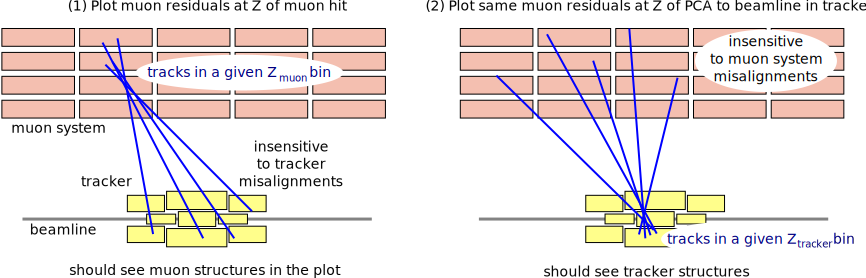
\includegraphics[width=\linewidth]{track_selection.png}

\begin{itemize}
\item To eliminate multiple scattering and $\vec{B}$ errors, select $|\vec{p}| > 40$~GeV
\item All plots made with the latest CRAFT constants
\end{itemize}
\end{frame}

\begin{frame}
\frametitle{Expansion/compression in $z$}

\begin{columns}
\column{0.66\linewidth}
\begin{itemize}\setlength{\itemsep}{-0.1 cm}
\item Plot on the right: $z$ residuals vs.\ $Z_{\mbox{\scriptsize muon}}$ at 550 $<$ $R$ $<$ 660~cm from beamline \mbox{(station 3)\hspace{-1 cm}}
\item Bottom 3 plots: same muon \mbox{resids vs.\ $Z_{\mbox{\scriptsize tracker}}$\hspace{-1 cm}}

\item We see a shift of TEC relative to TOB on bottom
  \mbox{\scriptsize ($y$ $<$ 0)} but not top \mbox{\scriptsize ($y$ $>$ 0)},
  indicates $z$ translation and $\phi_x$ rotation

\item 10~mm seen in station 3 $\Longrightarrow$ 1~mm \mbox{in TEC\hspace{-1 cm}}

\item Effect is more distinct in {\it outer} tracker

\vspace{-0.1 cm}
($R_{\mbox{\scriptsize PCA}}$ $>$ 60~cm), implicating TEC, \mbox{not TID\hspace{-1 cm}}
\end{itemize}

\column{0.33\linewidth}
\includegraphics[width=\linewidth]{zresid_from_muon.png}
\end{columns}

\vspace{0.2 cm}
\begin{columns}
\column{0.33\linewidth}
\scriptsize vs.\ $z$ in outer \mbox{tracker bottom\hspace{-1 cm}}

\includegraphics[width=\linewidth]{zresid_from_tracker_outerbottom.png}
\column{0.33\linewidth}
\scriptsize vs.\ $z$ in outer tracker top

\includegraphics[width=\linewidth]{zresid_from_tracker_outertop.png}
\column{0.33\linewidth}
\scriptsize vs.\ $z$ in inner tracker bottom

\includegraphics[width=\linewidth]{zresid_from_tracker_innerbottom.png}
\end{columns}
\end{frame}

\begin{frame}
\frametitle{Rotation around the beamline}

\begin{columns}
\column{0.66\linewidth}

\begin{itemize}
\item Below: $\phi_z$ (rotation around beamline) \mbox{residual\hspace{-0.5 cm}}
vs.\ $z$ in muon system; right: \mbox{same in tracker\hspace{-1 cm}}

\item Part of the rotation seen in the muon system is a real misalignment,
  indicated by the discontinuities at the wheel boundaries;
  slope within wheels caused by external bias

\item TIB/TOB has a large rotation, 0.5~mrad, and a
  small twist, 0.1-0.2~mrad end-to-end; vertical tracks may be between \mbox{TID/TEC layers\hspace{-1 cm}}
\end{itemize}

\column{0.33\linewidth}
\scriptsize $\phi_z$ resid vs.\ inner tracker $z$

\includegraphics[width=\linewidth]{phiresid_from_tracker_inner.png}
\end{columns}

\vspace{0.1 cm}
\begin{columns}
\column{0.66\linewidth}
\scriptsize \mbox{ } \hfill $\phi_z$ resid vs.\ muon $z$ (twist) \hfill \mbox{ }

\includegraphics[width=\linewidth]{phiresid_from_muon.png}

\column{0.33\linewidth}
\scriptsize $\phi_z$ resid vs.\ outer tracker $z$

\includegraphics[width=\linewidth]{phiresid_from_tracker_outer.png}
\end{columns}
\end{frame}

\begin{frame}
\frametitle{Sensitivity to tracker weak modes}

\vspace{0.2 cm}
\begin{columns}
\column{0.66\linewidth}
\begin{itemize}
\item Zijin prepared distortions of the tracker CRAFT alignment with an extra
  \mbox{$z$-expansion\hspace{-0.5 cm}} (stretch $z$ as a linear function of $z$) and twist
  ($\phi_z$ rotation as a function of $z$)
\item We reproduced the muon residuals versus $Z_{\mbox{\scriptsize tracker}}$ plots with these \mbox{tracker geometries\hspace{-1 cm}}
\item Extra twist is observable (two plots below), the 0.1\% $z$-expansion isn't (two on right)
\end{itemize}

\column{0.33\linewidth}
\scriptsize $z$ resid vs.\ inner tracker $z$

\includegraphics[width=\linewidth]{resid_from_tracker_inner_zexpand.png}
\end{columns}

\vspace{0.2 cm}
\begin{columns}
\column{0.33\linewidth}
\scriptsize $\phi_z$ resid vs.\ inner tracker $z$

\includegraphics[width=\linewidth]{phiresid_from_tracker_inner_twist2.png}
\column{0.33\linewidth}
\scriptsize $\phi_z$ resid vs.\ outer tracker $z$

\includegraphics[width=\linewidth]{phiresid_from_tracker_outer_twist2.png}
\column{0.33\linewidth}
\scriptsize $z$ resid vs.\ outer tracker $z$

\includegraphics[width=\linewidth]{resid_from_tracker_outer_zexpand.png}
\end{columns}
\end{frame}

\begin{frame}
\frametitle{Uncovered tracking problem}
\begin{itemize}
\item The $z$ compression results differ from what we quoted in \mbox{the past few\hspace{-1 cm}}
  weeks because means of $z$ residuals had been skewed by \mbox{rare large values\hspace{-1 cm}}
\begin{itemize}
\item effect is independent of momentum, so ``extrapolation to
  infinite momentum'' method didn't eliminate it
\item adds positive residuals on minus side and negative residuals on plus side: exaggerates CMS contraction
\item affected both HIP and MillePede algorithms equally, which is a
  clue because we do the refitting using slightly different tools
\end{itemize}
\item We will follow up on this
\end{itemize}

\vfill
\begin{columns}
\column{0.33\linewidth}
\scriptsize Old wheel -2 \mbox{``Alignment Plot''\hspace{-1 cm}}

\includegraphics[width=\linewidth]{oprof_whm2_nocut.pdf}

\column{0.33\linewidth}
\scriptsize Same with $|z_{\mbox{\tiny resid}}| < 200$~mm

\includegraphics[width=\linewidth]{oprof_whm2_withcut.pdf}

\column{0.33\linewidth}
\scriptsize $|q/p_T| < 0.05$~GeV$^{-1}$ bins

\includegraphics[width=\linewidth]{oparameter_whm2.pdf}
\end{columns}
\end{frame}

%% \section*{First section}
%% \begin{frame}
%% \begin{center}
%% \Huge \textcolor{blue}{First section}
%% \end{center}
%% \end{frame}

\begin{frame}
\frametitle{Conclusions}
\begin{itemize}\setlength{\itemsep}{0.05 cm}
\item Surprises in muon track-based alignment has inspired deeper
  diagnostic studies
\item Summary of preliminary conclusions presented in these slides
\begin{itemize}\setlength{\itemsep}{0.05 cm}
\item Muon wheels $\pm$2 want to {\it expand} 19~mm relative to CRAFT constants? (not expected: maybe ``ideal'' doesn't \mbox{represent $\vec{B}=0$?)\hspace{-1 cm}}
\item TEC appears to be misaligned about 1~mm in $z$
\item Tracker is rotated 0.5~mrad relative to muon system with a
  0.1-0.2~mrad end-to-end twist in the barrel; unsure \mbox{about endcap\hspace{-1 cm}}
\item Minus side of muon system has at least 1.0~mrad of real
  rotation; the rest may be due to external biases \mbox{(TEC rotation?\hspace{-0.3 cm}} an
  unidentified tracking error?)
\item We can easily see a 0.6~mrad end-to-end twist in the tracker
  barrel with this method, but not a 0.1\% $z$-expansion
\item Something gives rare refitted tracks large $z$ residuals,
  independent of $p_T$ but antisymmetric with $\eta$
\end{itemize}
\item Reminder: track-based alignment was not used to determine muon
  geometry for CRAFT re-processing; this is about improving it for next time
\end{itemize}
\end{frame}

\begin{frame}
\frametitle{Unraveling misalignments}

A proposal for correcting coupled tracker-muon misalignments by hand:

\vspace{-0.1 cm}
\begin{enumerate}
\item Fix the straight-forward misalignments, visible as discontinuities
\begin{itemize}\setlength{\itemsep}{0.1 cm}
\item rotate wheels to get a smooth curve in $\phi_z$ residual vs.\ $Z_{\mbox{\scriptsize muon}}$
\item TEC $z$ shift/$\phi_x$ angle: rotate such that the top is a fixed point and the bottom swings inward or outward
\begin{itemize}\setlength{\itemsep}{0.1 cm}
\item generate tracker geometries with $+$1 and $-$1~mm shift
\item find the sign that improves residuals vs.\ $Z_{\mbox{\scriptsize tracker}}$ and scale magnitude of final correction from response
\end{itemize}
\end{itemize}

\item See if there are still smooth trends in $\phi_z$ residual vs.\ $Z_{\mbox{\scriptsize muon}}$ \mbox{and $Z_{\mbox{\scriptsize tracker}}$\hspace{-1 cm}}
\begin{itemize}\setlength{\itemsep}{0.1 cm}
\item if so, interpret $\phi_z$ residual vs.\ $Z_{\mbox{\scriptsize tracker}}$ as real and untwist it
\item see if $\phi_z$ residual vs.\ $Z_{\mbox{\scriptsize muon}}$ is still present
\end{itemize}

\item See if wheel-by-wheel $z$ contraction is still large and \mbox{negative (expansion)\hspace{-1 cm}}
\begin{itemize}\setlength{\itemsep}{0.1 cm}
\item try putting in the largest $z$-expansion the tracker can
  tolerate, given the measured bounds (is this 0.1\% close to the limit?)
\end{itemize}

\item \ldots

\end{enumerate}
\label{numpages}
\end{frame}

\end{document}
